\documentclass{article}

\usepackage{neurips_2026}

\usepackage[utf8]{inputenc}
\usepackage[T2A,T1]{fontenc}
\usepackage[english,russian]{babel}
\usepackage{tempora}
\usepackage{hyperref}
\usepackage{url}
\usepackage{booktabs}
\usepackage{amsfonts}
\usepackage{amssymb}
\usepackage{amsmath}
\usepackage{nicefrac}
\usepackage{microtype}
\usepackage{xcolor}
\usepackage{graphicx}
\usepackage{array}
\usepackage{enumitem}
\usepackage{placeins}

\newcommand{\method}[1]{\texttt{#1}}
\newcommand{\wstar}{W^{\star}}
\newcommand{\mstar}{M^{\star}}
\newcommand{\cstar}{C^{\star}}

% TODO(camera-ready): venue retarget — this skeleton uses the NeurIPS 2026
% style shared by the companion papers; retarget to ICLR 2027 / AAMAS 2027
% class before submission.

\title{Семантический варп: завершение, обусловленное происхождением\\свидетельств, в коллективной памяти}

%\author{%
%  Anonymous Authors \\
%  Anonymous Institution \\
%  \texttt{anonymous@anonymous.edu} \\
%}

\begin{document}

\maketitle

\begin{abstract}
\textbf{Задача.} В коллективной памяти для многоагентной навигации агент может принять обязательство по цели --- и достичь её, --- ни разу её не наблюдав: все подтверждающие свидетельства пришли от соседей. Народная культура называет это навигацией по чужой песне; мы называем это \emph{семантическим варпом} (semantic warp). Метрики, учитывающие только успех, и даже постадийные метрики этого не видят, поскольку ни одна существующая методика оценки не обусловливает завершение (completion) \emph{происхождением} (provenance) свидетельств, стоящих за принятым обязательством.
\textbf{Подход.} Мы определяем событие варпа $\wstar_\theta := \mstar \wedge (\varphi \ge \theta)$, где чужеродность (foreignness) $\varphi$ --- это доля соседей в массе свидетельств, \emph{взятая в тех же весах, которыми слияние отбирало кандидата}, и зафиксированная в момент лока (lock). Варп --- не пятая стадия Q/R/M/C, а аннотация, расщепляющая $P(\cstar|\mstar)$ на страты по происхождению. Поскольку символьные слияния разлагаются по источникам, мы получаем (i) контрфактическую атрибуцию ценности варпа через детерминированный повтор с маскированием чужих свидетельств, (ii) \emph{закон варп-дистанции} в замкнутой форме, выведенный из правил доверие$\times$устаревание (trust$\times$staleness), и (iii) децентрализованный протокол \emph{Warp Drive} (оптимистичный лок + резервация + анти-$\mstar$-откат) для патологии варп-коллизий.
\textbf{Результаты.} На развёртке дефицита из 2{,}400 эпизодов сырые варп-локи почти никогда не завершаются напрямую ($P(\cstar|\wstar)=0.004$--$0.020$ против $0.22$--$0.41$ для собственных локов; доверительные интервалы не пересекаются), однако чужие свидетельства всё же несут ценность как транспорт: до $51\%$ завершений собственных локов --- это варп-ассистированные цепочки. Закон дистанции предсказывает горизонты формирования намерения с точностью до такта, включая отложенную проверку $6/6$ с предсказаниями, зарегистрированными до исполнения. Warp Drive разворачивает компромисс: доля успеха растёт при каждой каденции (cadence) с непересекающимися интервалами, и быстрый обмен с протоколом обходит лучший базовый вариант с фиксированной каденцией ($0.614$--$0.620$ против $0.583$). Строгий межсессионный и межагентный варп воспроизведён на LLM-субстрате ($10/10$ планировок против $0/10$ без чужой памяти).
\textbf{Тезис.} Ценность коллективной памяти состоит не столько в самой информации, сколько в \emph{координационном контракте, прикреплённом к информации}.
\textbf{Границы.} Сеточные субстраты и одна небольшая текстовая LLM-демонстрация; вклад --- измерительный слой, фальсифицируемый закон и минимальный протокол, а не общая теория.
\end{abstract}

\section{Введение}
\label{sec:intro}

В культурах песенных троп путник, знающий песню, способен пересечь
местность, которой никогда не видел: навигационная компетентность
передаётся без физического посещения. Многоагентные системы с общей
памятью совершают тот же акт постоянно --- агент принимает
обязательство по источнику воды, целевой области или расположению
инструмента, известным лишь из широковещательной рассылки соседа, ---
однако ни одна стандартная методика оценки не отличает этот акт от
обычной навигации по памяти. Метрики успеха агрегируют поверх него;
постадийная диагностика вроде Q/R/M/C считает обязательство
($\mstar$) и завершение ($\cstar$), но не то, \emph{чьи свидетельства}
их подкрепили.

Эта статья делает такой акт полноправным измеряемым событием.
\emph{Семантический варп} $\wstar$ --- это материализация цели, масса
подтверждающих свидетельств которой (почти) целиком чужеродна, а
\emph{завершение варпа} $P(\cstar|\wstar)$ спрашивает, доводит ли
чужая песня действительно до места. Три свойства символьной
коллективной памяти делают конструкцию строгой, и ни одно из них не
выполняется для непрозрачных векторных памятей:

\begin{enumerate}[leftmargin=20pt,itemsep=2pt,topsep=2pt]
\item \textbf{Слияния разлагаются по источникам.} Чужеродность
  $\varphi\in[0,1]$ вычисляется из тех же по-источниковых весов
  (доверие, устаревание, поддержка), которыми само слияние
  ранжировало кандидата --- это прочтение решения, а не новая
  эвристика.
\item \textbf{Повторы детерминированы.} Повторный прогон эпизода с
  маскированием чужих вкладов на этапе слияния даёт
  \emph{контрфактический} выигрыш варпа для каждого эпизода, а не
  корреляцию.
\item \textbf{Правила обмена имеют замкнутую форму.} Затухание
  доверия и устаревания влечёт \emph{закон варп-дистанции}: явный
  горизонт, за которым чужие свидетельства уже не могут формировать
  намерение --- фальсифицируемый и фальсифицируемо различный у разных
  архитектур.
\end{enumerate}

Наши измерения затем вынуждают переосмысление. Сырой варп почти
бесполезен в точке завершения: при дефиците варп-локи завершаются на
порядок реже, чем локи на собственных свидетельствах
(\S\ref{sec:raw}), потому что одновременные получатели одной и той же
рассылки соревнуются за одну цель, и большинство обречено проиграть.
Однако те же чужие свидетельства доказуемо ценны как
\emph{транспорт}: до половины всех завершений на собственных
свидетельствах --- это цепочки, начавшиеся с провалившегося
варп-лока, который довёз агента до зоны самоподтверждения
(\S\ref{sec:taxi}). А лёгкий децентрализованный контракт ---
резервация, подсаженная на уже существующую рассылку, плюс
анти-$\mstar$-откат в духе симуляций Time
Warp~\cite{jefferson1985}
--- возвращает то, что теряет сырой варп: с протоколом \emph{быстрый}
обмен становится лучшим режимом по безусловной доле успеха
(\S\ref{sec:drive}). Отсюда тезис в одном предложении:
\textbf{ценность коллективной памяти --- не информация, а
координационный контракт, прикреплённый к информации.}

\paragraph{Вклад работы.}
\begin{enumerate}[leftmargin=20pt,itemsep=2pt,topsep=2pt]
\item Первая метрика завершения, обусловленная происхождением
  свидетельств, для коллективной памяти: $\wstar_\theta$, $\varphi$,
  замороженная в момент лока, разложение
  $P(\cstar|\mstar)=P(\cstar|\mstar,\varphi{<}\theta)\,P(\varphi{<}\theta|\mstar)
  + P(\cstar|\wstar)\,P(\wstar|\mstar)$ и контрфактический выигрыш
  варпа через детерминированный повтор с маскированием источников
  (\S\ref{sec:warp-def}--\S\ref{sec:raw}).
\item \emph{Закон варп-дистанции}
  $\mathrm{age}_{\max}(\tau_i)=\alpha^{-1}\ln(\tau_i c/\tau)$,
  выведенный из собственных правил доверие$\times$устаревание самой
  памяти, подтверждённый с точностью до такта, включая отложенную
  проверку с зарегистрированными предсказаниями ($6/6$ точных, в том
  числе ячейка, где горизонт отсечки обязан сработать раньше
  экспоненциального гейта --- и срабатывает), и различие формы на
  уровне архитектур: у пиринговой памяти с фиксированной каденцией
  гейта \emph{нет} (\S\ref{sec:law}).
\item Протокол \emph{Warp Drive}: оптимистичный варп-лок, резервации,
  переносимые на существующей каденции рассылки (без координатора), и
  анти-$\mstar$-откат с экспоненциальной выдержкой. Он превентивно
  разрешает известную патологию введённого в заблуждение агента,
  ограничивает задержку отката величиной ${\approx}K$ тактов и
  поднимает безусловную долю успеха выше лучшего базового варианта с
  фиксированной каденцией (\S\ref{sec:drive}).
\item Строгий межсессионный, межагентный варп на LLM-субстрате:
  агент, никогда не наблюдавший комнату, решает там задачу
  исключительно по памяти другого агента из предыдущей сессии;
  воспроизведено на $10/10$ планировках против контроля $0/10$
  (\S\ref{sec:llm}).
\end{enumerate}

\paragraph{Связь со статьями-компаньонами.}
Статья о фреймворке Q/R/M/C рассматривает постадийные показатели как
измерительный инструмент; статья о коллективной памяти устанавливает
архитектуры и компромисс каденции. Настоящая статья добавляет поверх
обеих ось происхождения: те же логи, одна новая аннотация и
механизмы, которые эта аннотация обнажает. % TODO: cite companions per venue policy.

\section{Постановка}
\label{sec:setting}

\paragraph{Субстрат и задача.} $N$ агентов исследуют сетку
$12\times10$ с $M$ семантическими целями-водоёмами ($N>M$: дефицит) и
опасностями. Каждый агент поддерживает символьную память мест (теги,
уверенности, поддержка, свежесть). Четыре архитектуры обмена поверх
идентичного субстрата и планировщика: \method{independent} (без
коммуникации), \method{shared} (единая шина событий),
\method{centralized} (консенсусный агрегатор), \method{peer}
(рассылка каждые $K$ тактов, асимметричное доверие), плюс
\method{CSM} (peer $+$ явные правила слияния/доверия/устаревания со
скоростью затухания $\alpha{=}0.05$ и порогом включения
$\tau{=}0.30$). % TODO: compress substrate details; cite companion §2.

\paragraph{Инструментирование Q/R/M/C.} На каждом такте для каждого
агента логируются формирование запроса (Q), удовлетворение выборки
(R), материализация цели как лок планировщика ($\mstar$) и завершение
($\cstar$). Условные показатели уровня эпизода следуют определению из
статьи-компаньона. Все измерения варпа ниже --- аннотации этих
событий $\mstar$; ни один инвариант планировщика или памяти не
изменяется.

\section{Событие варпа}
\label{sec:warp-def}

\paragraph{Происхождение и чужеродность.} Каждая единица
свидетельства, входящая в слияние, несёт свой источник. Для
кандидата $m$, на котором планировщик ставит лок,
\[
\varphi(m) \;=\;
\frac{\sum_{e\in\mathrm{supp}(m),\,\pi(e)\neq\mathrm{self}} w(e)}
     {\sum_{e\in\mathrm{supp}(m)} w(e)},
\]
где $w(e)$ --- \emph{собственные веса слияния}: $\text{trust}\cdot
\log(1{+}\text{support})$ для консенсуса peer/centralized,
$\text{trust}\cdot e^{-\alpha\,\text{age}}\cdot\text{conf}$ для CSM,
массы наблюдений для общей шины. Для архитектур peer и centralized
$\varphi$ восстанавливается точно из повкладовых полей, которые
слияние уже экспортирует; измерительный слой читает состояние и
никогда его не пишет.

\paragraph{Правило заморозки.} $\varphi$ фиксируется в момент лока.
Если агент позже подтверждает место собственными глазами, $\varphi$
\emph{не} пересчитывается --- иначе каждый успешный варп размывал бы
сам себя на подходе, и $P(\cstar|\wstar)$ была бы неизмерима по
построению.

\paragraph{События варпа и страты.} $\wstar_\theta := \mstar \wedge
(\varphi\ge\theta)$ при $\theta{=}1$ (строгий: цель ни разу не
наблюдалась самим агентом, что перекрёстно проверяется по журналу
наблюдений) и $\theta{=}0.8$ (мягкий). Доля варпа $P(\wstar|\mstar)$
--- структурный дескриптор (тождественно $0$ для
\method{independent}); завершение варпа $P(\cstar|\wstar)$ --- новая
величина. Разложение по правилу цепочки из \S\ref{sec:intro} делает
варп точным уточнением $P(\cstar|\mstar)$, а не новой стадией:
идентифицируемость Q/R/M/C не затронута.

\paragraph{Регрессионный якорь.} Известный эпизод введённого в
заблуждение агента из сравнения архитектур (агент A ставит лок на
$(3,8)$, известную только от C; C занимает её первым; A застревает)
аннотируется инструментированием как строгий $\wstar$ с
$\varphi=1.0$ и коллизией --- патология, которую фреймворк обязан
видеть, а протокол из \S\ref{sec:drive} обязан чинить.

\section{Сырой варп редко завершается --- но перевозит}
\label{sec:raw}

\paragraph{Дизайн.} $2{,}400$ эпизодов: $(N,M)\in\{(3,2),(5,3),(8,5),
(4,4),(6,2)\}$ $\times$ три планировки $\times$
$\{\text{peer-}K2,\text{peer-}K8,\text{CSM-}K8,\text{shared}\}$
$\times$ 20 сидов $\times$ \{полный, с маскированием чужого\} при
идентичных сидах. Единица анализа: событие лока; доверительные
интервалы --- бутстреп с кластеризацией по эпизодам.

\begin{figure}[t]
\centering
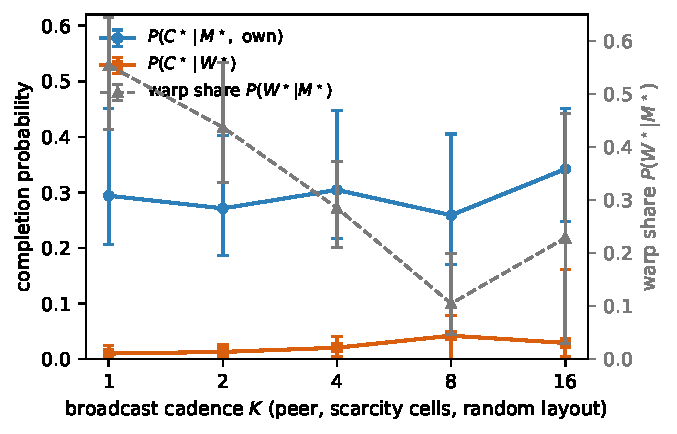
\includegraphics[width=0.72\linewidth]{figures/fig_warp_strata}
\caption{Завершение, стратифицированное по $\varphi$, в зависимости
от каденции рассылки $K$ (выделенная развёртка peer: ячейки дефицита,
случайные планировки, 20 сидов, бутстреп-интервалы с кластеризацией
по эпизодам). По мере уменьшения $K$ доля варпа $P(\wstar|\mstar)$
растёт с $0.11$ до $0.55$, тогда как $P(\cstar|\wstar)$ остаётся ниже
$0.05$, а показатель собственной страты не меняется: коллапс
завершения при быстром обмене сосредоточен в страте $\wstar$, что
даёт механистическое прочтение сдвигу узкого места из
статьи-компаньона. Подскок доли при $K{=}16$ (рассылки редки, но и
сами агенты мало что открывают) приводится как наблюдённый.}
\label{fig:strata}
\end{figure}

Рисунок~\ref{fig:strata} показывает каденционный срез на выделенной
развёртке peer ($K\in\{1,2,4,8,16\}$): доля варпа --- это то, что
покупает быстрый обмен, и это ровно та страта, которая не
завершается. Таблица~\ref{tab:hw1} даёт срез по архитектурам.

\begin{table}[h]
\centering
\caption{Страты завершения по происхождению при дефиците ($N>M$),
полные прогоны. Варп-локи завершаются на порядок реже, чем локи на
собственных свидетельствах; все пары доверительных интервалов не
пересекаются. (H-W1 подтверждена.)}
\label{tab:hw1}
\small
\begin{tabular}{lcccc}
\toprule
Архитектура & $P(\cstar|\wstar_{0.8})$ & $n_{\wstar}$ & $P(\cstar|\mstar,\text{own})$ & $n_{\text{own}}$ \\
\midrule
peer-$K{=}2$ & 0.004 [0.001, 0.008] & 1{,}437 & 0.223 [0.186, 0.275] & 2{,}738 \\
peer-$K{=}8$ & 0.020 [0.000, 0.038] & 149    & 0.389 [0.329, 0.446] & 1{,}734 \\
CSM-$K{=}8$  & 0.017 [0.006, 0.044] & 637    & 0.414 [0.368, 0.453] & 1{,}684 \\
shared       & 0.004 [0.002, 0.008] & 2{,}099 & 0.279 [0.237, 0.332] & 2{,}250 \\
\bottomrule
\end{tabular}
\end{table}

\subsection{Варп как транспорт: цепочки локов}
\label{sec:taxi}

Прямое завершение недооценивает ценность чужих свидетельств.
\emph{Варп-ассистированное собственное завершение} --- это
завершённый лок на собственных свидетельствах, которому (у того же
агента, в том же эпизоде) предшествовал сброшенный мягкий
$\wstar$-лок: варп провалился как пункт назначения, но удался как
поездка.

\begin{table}[h]
\centering
\caption{Анализ цепочек локов (случайные планировки, полные прогоны).
Первый $\wstar$-лок в цепочке ставится с расстояния
${\approx}8$--$10$ клеток; завершающий собственный лок --- с $2.0$
клеток, то есть ровно с радиуса наблюдения, точки
самоподтверждения.}
\label{tab:taxi}
\small
\begin{tabular}{lccc}
\toprule
Ветвь & собств. $\cstar$ & варп-ассистированные (доля) & $r(\text{first }\wstar) \to r(\text{own})$ \\
\midrule
shared          & 248 & 127 (\textbf{51.2\%}) & $9.5 \to 2.0$ \\
peer-$K{=}2$    & 223 & 99 (\textbf{44.4\%})  & $9.7 \to 2.0$ \\
CSM-$K{=}8$     & 279 & 13 (4.7\%)            & $5.8 \to 2.0$ \\
peer-$K{=}8$    & 246 & 7 (2.8\%)             & $8.4 \to 2.0$ \\
\bottomrule
\end{tabular}
\end{table}

Это разрешает кажущийся парадокс контрфактических данных: общая шина
при умеренном дефиците выигрывает от чужих свидетельств $+10.8$ такта
$[+2.2,+20.9]$, хотя её прямое $P(\cstar|\wstar)$ равно $0.004$.
Выигрыш течёт через цепочки; правило заморозки честно записывает
завершение в собственную страту, а анализ цепочек восстанавливает
вклад варпа как отдельную измеренную величину.

\subsection{Контрфактический выигрыш варпа}
\label{sec:gain}

Маскирование чужих свидетельств на этапе слияния при том же сиде даёт
$\mathrm{WG} = t_{\text{cens}}(\text{masked}) -
t_{\text{cens}}(\text{full})$ на эпизод. Карта знаков по (планировка,
дефицит $\rho{=}N/M$) зависит от режима: положительна для общей шины
на непредсказуемых планировках при умеренном дефиците ($+10.8$ при
$\rho{=}1.5$), отрицательна для быстрого пирингового обмена
(peer-$K2$, случайные планировки: $-7.1$ $[-13.5,-1.3]$),
${\approx}0$ при жёстком дефиците. Поагентная маска (один агент
маскирован, остальные обмениваются как обычно) подтверждает знак на
индивидуальном уровне: $\mathrm{WG}_i = -10.25$ $[-20.91,-0.16]$
такта на ячейке быстрого обмена при дефиците, при этом побочный
эффект на немаскированных агентах ${\approx}0$ ($-0.62$
$[-3.06,+1.91]$). Сырой варп \emph{вредит} своему получателю ровно
там, где обмен самый быстрый --- цена коллизий превышает ценность
информации. % TODO: full sign map to appendix.

\paragraph{Разведочный результат: давление коллизий.} Давление
со-локов (другие агенты, залоченные на ту же цель) коррелирует с
провалом варпа с предсказанным знаком, но пренебрежимой величиной
(Спирмен $+0.033$, $p{=}0.018$, $n{=}5{,}117$); мы приводим это как
разведочный результат, а не как подтверждённый предиктор.
% honest downgrade of pre-registered H-W5

\section{Закон варп-дистанции}
\label{sec:law}

CSM включает чужое свидетельство с весом $\tau_i\, e^{-\alpha\,
\text{age}}\, c$ (доверие $\tau_i$, уверенность $c{=}0.95$) и порогом
включения $\tau{=}0.30$. Следовательно, чужое свидетельство перестаёт
формировать намерение при
\[
\mathrm{age}_{\max}(\tau_i) \;=\; \tfrac{1}{\alpha}\,
\ln\!\big(\tau_i\, c / \tau\big), \qquad \text{определено при } \tau_i c > \tau .
\]

\paragraph{Протокол «свидетель--путник».} Свидетель один раз
наблюдает воду и замолкает; путник, никогда её не видевший, получает
снимок памяти с параметризованным возрастом. Каждый лок путника ---
строгий $\wstar$ по построению. Рисунок~\ref{fig:law} суммирует оба
эксперимента.

\begin{figure}[t]
\centering
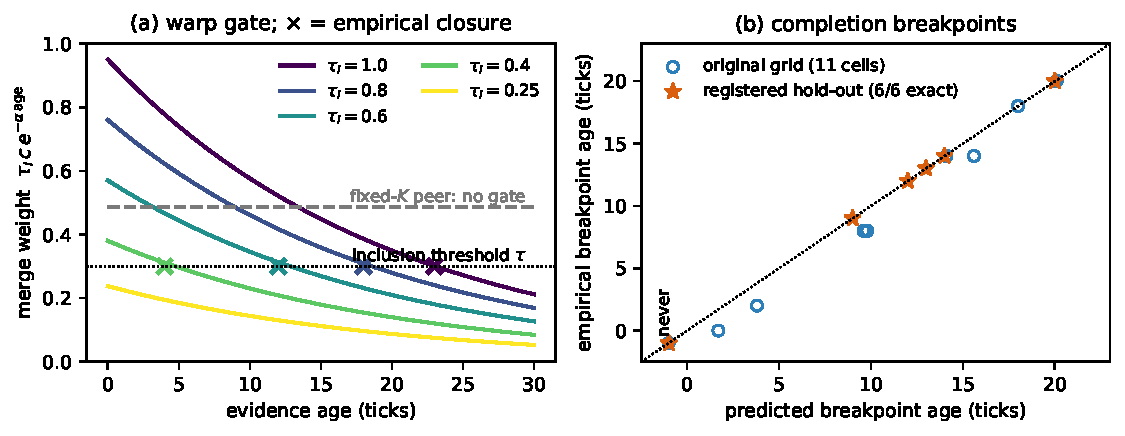
\includegraphics[width=\linewidth]{figures/fig_warp_law}
\caption{Закон варп-дистанции. \textbf{(a)} Вес чужого свидетельства
в слиянии при затухании доверие$\times$устаревание; $\times$ отмечает
эмпирически измеренный последний возраст, при котором запрос путника
ещё обнажает цель --- каждый лежит на пересечении своей кривой с
порогом включения $\tau$. У пиринговой памяти с фиксированной
каденцией члена устаревания нет (пунктир): её гейт никогда не
закрывается; архитектуры различаются \emph{формой} кривой.
\textbf{(b)} Предсказанные и эмпирические точки излома завершения в
полных навигационных эпизодах: исходная сетка (кружки; возраст
дискретизован с шагом 2, поэтому точки лежат не более чем на один шаг
сетки ниже диагонали) и зарегистрированная отложенная проверка
(звёздочки; шаг возраста 1, предсказания записаны на диск до
исполнения, $6/6$ точных, включая never-ячейку в $(-1,-1)$ и ячейку,
где горизонт отсечки срабатывает раньше экспоненциального гейта).}
\label{fig:law}
\end{figure}

\begin{table}[h]
\centering
\caption{Кривая гейта: наибольший возраст свидетельства, при котором
запрос путника ещё обнажает цель. У пиринговой памяти с фиксированной
каденцией члена устаревания нет: гейт никогда не закрывается
(проверено до возраста 120 при всех уровнях доверия) --- архитектуры
различаются \emph{формой} кривой, а не только её уровнем.}
\label{tab:gate}
\small
\begin{tabular}{lcc}
\toprule
доверие $\tau_i$ & эмпирический $\mathrm{age}_{\max}$ & предсказание \\
\midrule
1.00 & 23 & 23.05 \\
0.80 & 18 & 18.59 \\
0.60 & 12 & 12.84 \\
0.40 & 4  & 4.73 \\
0.25 & гейт закрыт & 0 (trust-flip) \\
\bottomrule
\end{tabular}
\end{table}

\paragraph{Точка излома завершения.} В полных навигационных эпизодах
неравенство осуществимости получает одно дискретное уточнение: путник
самоподтверждает цель, как только она оказывается в радиусе
наблюдения, поэтому чужому гейту достаточно продержаться до такта
$t_{\text{gate}} = d - r_{\text{obs}} - 1$, что даёт точку излома
$\mathrm{bp} = \mathrm{age}_{\max} - t_{\text{gate}}$; отсечка
снимков исполняется на тактах рассылки и добавляет границу $10K -
t_{\text{bcast}}$. Все константы закона неизменны. Все 11 ячеек CSM
исходной сетки совпадают в пределах разрешения дискретизации; кривые
завершения --- монотонные ступени; trust-flip дискретно обнуляет
события $\wstar$.

\begin{table}[h]
\centering
\caption{Отложенная проверка с зарегистрированными предсказаниями:
шесть ячеек, отсутствующих в исходной сетке, предсказания записаны на
диск \emph{до} любого эпизода, шаг сетки возраста 1. Все шесть ---
точные целочисленные совпадения, включая never-ячейку и ячейку, где
горизонт отсечки обязан сработать раньше экспоненциального гейта.}
\label{tab:holdout}
\small
\begin{tabular}{lccc}
\toprule
Ячейка & связывающая граница & предсказание & эмпирика \\
\midrule
$K{=}8$, $\tau_i{=}0.9$, $d{=}9$  & гейт    & 14 & \textbf{14} \\
$K{=}8$, $\tau_i{=}0.7$, $d{=}9$  & гейт    & 9  & \textbf{9}  \\
$K{=}8$, $\tau_i{=}0.5$, $d{=}15$ & гейт    & никогда & \textbf{никогда} \\
$K{=}4$, $\tau_i{=}1.0$, $d{=}6$  & гейт    & 20 & \textbf{20} \\
$K{=}2$, $\tau_i{=}1.0$, $d{=}12$ & \emph{отсечка} & 12 & \textbf{12} \\
$K{=}2$, $\tau_i{=}0.8$, $d{=}8$  & гейт    & 13 & \textbf{13} \\
\bottomrule
\end{tabular}
\end{table}

Закон, таким образом, предсказателен вне выборки с точностью до
такта: правила CSM действительно являются механизмом, который
формирует (и расформировывает) намерение. Он также переинтерпретирует
результат статьи-компаньона о том, что CSM доминирует над пиринговой
памятью с фиксированной каденцией: доверие$\times$устаревание --- это
\emph{варп-гейт} --- CSM не обменивается лучше, она \emph{отказывается
варпать по устаревшей или недоверенной песне}.

\paragraph{Переносимость на непрерывную динамику.} Все три
зарегистрированных предсказания выживают на непрерывном субстрате
VMAS через тот же мост «непрерывное$\to$сетка», что и в тесте
переносимости статьи-компаньона: (i) страты по происхождению остаются
разнесёнными на порядок ($P(\cstar|\wstar)=0.012$ $[0.000,0.042]$
против $0.562$ $[0.457,0.709]$ при $K{=}1$); (ii) доля варпа
монотонно падает с каденцией ($0.723\to0.366\to0.000$ по $K{=}1/4/16$);
(iii) закон становится \emph{метрическим}: при однократной калибровке
времени «путь до видимости» на эпизоде со свежим свидетельством
предсказанные точки излома совпадают в пределах сетки дискретизации,
а все ячейки за метрическим радиусом варпа
($v\cdot\mathrm{age}_{\max}$ короче расстояния) предсказаны как
\emph{никогда} и наблюдены как \emph{никогда}. Один по-настоящему
непрерывный вывод: инерция --- физический канал утечки варпа --- агент
может по инерции вкатиться в зону видимости после закрытия гейта;
устраняется контроллером «нет лока --- тормози», восстанавливающим
сеточную семантику.

\section{Протокол Warp Drive}
\label{sec:drive}

Варп-коллизия --- лок на чужих свидетельствах по цели, которую займёт
кто-то другой, --- доминирующий отказ быстрого обмена. Warp Drive
добавляет три примитива, все децентрализованные:

\begin{enumerate}[leftmargin=20pt,itemsep=2pt,topsep=2pt]
\item \textbf{Оптимистичный варп-лок} --- локи на чужих
  свидетельствах остаются разрешены немедленно (планировщик не
  изменяется).
\item \textbf{Варп-резервация} --- на ближайшем такте рассылки
  владельца резервация едет на обычном снимке (та же каденция $K$,
  без координатора, без дополнительного канала); получатели подавляют
  зарезервированные цели в своих запросах. Приоритет: (такт лока,
  расстояние в момент лока, идентификатор агента).
\item \textbf{Анти-$\mstar$-откат} (семантика Time
  Warp~\cite{jefferson1985}) --- агент, чей лок доминирован чужой
  резервацией, отзывает его: планировщик перезапрашивает, цель уходит
  в экспоненциальную выдержку ($4\to8\to\cdots\to32$ тактов) с
  разрешением ничьих по идентификатору агента против осцилляций.
  Журнал событий остаётся только дополняемым (append-only).
\end{enumerate}

\paragraph{Проверка децентрализации.} Прогон протокола прямыми
поагентными вызовами --- без рантайма, без окружения --- даёт те же
решения об отзыве по одному лишь собственному входящему ящику каждого
агента.

\paragraph{Якорь «введённого в заблуждение A».} С Warp Drive
патологический лок разрешается \emph{превентивно}: резервация C
приходит до того, как A вообще залочится на $(3,8)$; A завершает на
другой цели. В развёртке задержка отката доминированных локов конечна
и составляет ${\approx}K$: $1.0/1.5/2.7$ такта при $K{=}1/2/4$
(базовый вариант: до конца эпизода).

\begin{figure}[t]
\centering
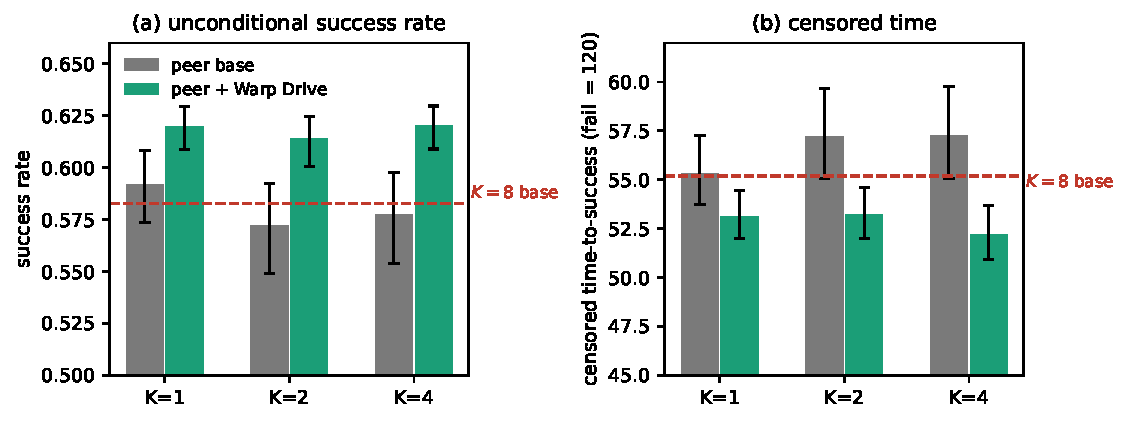
\includegraphics[width=\linewidth]{figures/fig_warp_drive}
\caption{Warp Drive на безусловных метриках (840 эпизодов;
бутстреп-интервалы). \textbf{(a)} Доля успеха растёт при каждой
каденции с непересекающимися интервалами, и каждая быстрая ветвь с
протоколом превосходит базовую «сладкую точку» $K{=}8$ (пунктир).
\textbf{(b)} Цензурированное время до успеха соответственно падает.
Утверждение о том, что протокол снимает главный аргумент против
быстрого обмена, опирается на эти безусловные величины, а не на
(чувствительные к знаменателю) условные показатели.}
\label{fig:drive}
\end{figure}

\begin{table}[h]
\centering
\caption{Безусловные результаты, 840 эпизодов (ячейки дефицита
$\times$ случайные/асимметричные планировки $\times$ 20 сидов). Доля
успеха под Warp Drive растёт при каждой каденции с непересекающимися
интервалами, цензурированное время падает, и быстрый обмен с
протоколом обходит базовую «сладкую точку» $K{=}8$
(рисунок~\ref{fig:drive}). Перепись локов показывает сжатие
знаменателя условных метрик --- поэтому утверждение сформулировано на
безусловных величинах.}
\label{tab:wd}
\small
\begin{tabular}{lccc}
\toprule
Ветвь & доля успеха & $t_{\text{cens}}$ (провал $=120$) & перепись локов \\
\midrule
$K{=}1$ базовый & 0.592 [0.574, 0.608] & 55.3 [53.7, 57.2] & 0.986 \\
$K{=}1$ +WD  & \textbf{0.620} [0.609, 0.629] & 53.1 [52.0, 54.4] & 0.985 \\
$K{=}2$ базовый & 0.572 [0.549, 0.592] & 57.2 [55.1, 59.7] & 0.973 \\
$K{=}2$ +WD  & \textbf{0.614} [0.601, 0.624] & \textbf{53.2} [52.0, 54.6] & 0.926 \\
$K{=}4$ базовый & 0.577 [0.554, 0.598] & 57.3 [55.1, 59.8] & 0.944 \\
$K{=}4$ +WD  & \textbf{0.620} [0.609, 0.630] & \textbf{52.2} [50.9, 53.7] & 0.739 \\
$K{=}8$ базовый & 0.583 [0.558, 0.604] & 55.2 [52.9, 57.9] & 0.682 \\
\bottomrule
\end{tabular}
\end{table}

На условной оси восстановление измеряется относительно потолка
дефицита $\min(m,M)/m$ (никакой протокол не наколдует лишней воды):
$0.90 / 2.15 / 6.6$ восстановимого коллапса при $K{=}1/2/4$; значения
выше 1 возникают потому, что подавление по резервациям убирает
обречённые локи из популяции $\mstar$. Вместе с
таблицей~\ref{tab:taxi} это замыкает дугу: сырой варп проваливается
на завершении (\S\ref{sec:raw}); с прикреплённым координационным
контрактом варп на быстрой каденции становится лучшим режимом.
«Сладкая точка» каденции из статьи-компаньона переинтерпретируется:
умеренный $K$ никогда не был про свежесть информации --- это был
неявный ограничитель частоты варп-коллизий, и явный контракт
справляется с этой работой лучше.

\section{Межсессионный варп на LLM-субстрате}
\label{sec:llm}

Наконец, строгий варп пересекает одновременно границу агента и
границу сессии на языковом субстрате. В сессии 1 агент A (локальный
LLM-экстрактор тегов над наблюдениями на естественном языке; Ollama
\method{llama3.1}, детерминированное кеширование, нулевая стоимость
API) обходит трёхкомнатный текстовый дом, и его символьная память
выгружается на диск. В сессии 2 агент B --- свежий агент в свежем
экземпляре окружения, из которого удалён штатный направляющий оракул,
так что дальнее знание может прийти только из памяти, --- загружает
дамп A как чужое происхождение и решает задачу «принеси яблоко на
стол». Каждый лок B на яблоке или столе --- строгий $\wstar$ с
$\varphi{=}1.0$; исполнение слоистое (LLM принимает семантические
решения --- какое запомненное место преследовать, когда взять/положить,
--- а перемещение к залоченной путевой точке выполняет
детерминированный моторный примитив, в соответствии со стеком
планировщика субстрата).

\begin{table}[h]
\centering
\caption{Межсессионный варп на 10 рандомизированных планировках.
Завершение засчитывается на радиусе аффорданса окружения (действие
взять/положить в пределах манхэттенского расстояния 1, и свидетель
помечает якоря на достижимых клетках).}
\label{tab:llm}
\small
\begin{tabular}{lccc}
\toprule
 & успех & среднее $t_{\text{succ}}$ & планировки с завершённым строгим $\wstar$ \\
\midrule
варп (память A) & \textbf{10/10} & 8.3 & \textbf{10/10} \\
контроль (пустая память) & 0/10 & --- & --- \\
\bottomrule
\end{tabular}
\end{table}

Насколько нам известно, это первый задокументированный межсессионный,
межагентный строгий семантический варп на LLM-субстрате. Контраст
$10/10$ против $0/10$ показывает, что варп несущий, а не
декоративный.

\paragraph{Масштабирование до живого коллектива.} При $N{=}3$
LLM-агентах, обменивающихся пиринговой рассылкой в условиях дефицита
($M{=}2$ яблока, четыре планировки, $K\in\{2,8\}$), вся
феноменология варпа воспроизводится на языковом субстрате (все
предсказания зарегистрированы до прогонов): строгие $\wstar$-локи
происходят; доля варпа падает с каденцией ($0.417$ при $K{=}2$ против
$0.083$ при $K{=}8$ --- та же форма, что и на сетке
$0.554\!\to\!0.105$ и в VMAS $0.723\!\to\!0.000$); варп-коллизии
появляются в $7/8$ эпизодов. Парное сравнение с базовым вариантом без
коммуникации на идентичных планировках показывает, что сырой обмен
\emph{снижает} успех с $2/3$ до $1/3$ на эпизод --- цена коллизий
превышает ценность информации на LLM-субстрате ровно как в
\S\ref{sec:gain}. Прикрепление неизменённого протокола Warp Drive к
LLM-коллективу замыкает дугу и на языке: суммарный успех растёт с
$0.333$ до $0.417$ на обеих каденциях, а задержки отката снова
${\approx}K$ ($1$ такт при $K{=}2$, $7$ при $K{=}8$). Восстановление
частично (${\approx}25\%$ коллапса против $90$--$100\%$ на сетке): на
языковом субстрате патология коллизий усугубляется потерями
семантического уровня (галлюцинированные якорные теги, шумные локи),
которые никакая резервация не лечит --- измеримое разложение мы
оставляем будущей работе. Закон дистанции также выдерживает
свидетельства, произведённые LLM: при константе гейта $c$, равной
уверенности, которую экстрактор реально выдал
($c_{\text{meas}}{=}0.900$), все четыре зарегистрированные точки
излома ложатся в пределах одного такта от предсказания.

Два вывода об интерфейсе переносятся на любой дизайн
«LLM поверх символьной памяти»: формирователь запросов на LLM свободно
генерирует поисковые теги вне словаря памяти (что требует гейта
any-of), а малые локальные модели надёжны в семантическом
обязательстве, но не в координатной арифметике и не в систематическом
исследовании (что требует описанного выше слоистого исполнения и
явного яруса исследования --- без него открытие не происходит, и варпу
нечем питаться).

\begin{figure}[t]
\centering
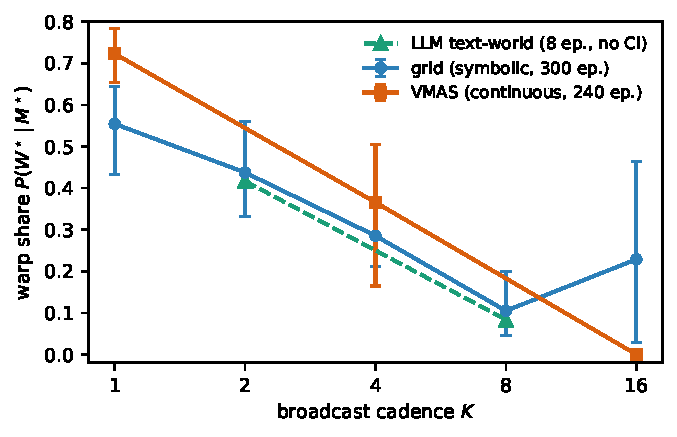
\includegraphics[width=0.62\linewidth]{figures/fig_warp_universality}
\caption{Одна величина, три субстрата: доля варпа $P(\wstar|\mstar)$
в зависимости от каденции рассылки $K$ на символьной сетке, в
непрерывном сценарии VMAS и в текстовом мире с LLM. Кривые почти
совпадают --- то, какая часть материализаций коллектива работает на
чужих свидетельствах, определяется каденцией обмена, а не субстратом.
(Ветвь LLM: 8 эпизодов, только точечные оценки.)}
\label{fig:universality}
\end{figure}

Рисунок~\ref{fig:universality} накладывает кривую «доля
варпа--каденция» по всем трём субстратам: величина ведёт себя как
свойство архитектуры обмена, свободное от субстрата.

\section{Связанные работы}
\label{sec:related}

\paragraph{Общая память в коллективах агентов.} Generative
Agents~\cite{park2023generative} и многоагентные LLM-фреймворки
разделяют потоки памяти или контекст, но не обнажают ни интерфейса
лока, ни по-источникового разложения слитого убеждения, так что
завершение, обусловленное происхождением, там неизмеримо. Векторные
памяти (например, MemGPT~\cite{packer2023memgpt}) сливают
арифметикой вложений; такое слияние не разлагается по источникам, что
блокирует и $\varphi$, и контрфактический повтор с маскированием.
\paragraph{Эмерджентная коммуникация.} CommNet~\cite{sukhbaatar2016commnet}
и TarMAC~\cite{das2019tarmac} обучают непрерывные каналы;
статья-компаньон показывает, что такие каналы схлопывают
наблюдаемость стадий. Варп требует явного события материализации,
которого эти архитектуры не обнажают.
\paragraph{Стигмергия.} Координация в стиле феромонов --- это
\emph{анонимный} варп: свидетельства передаются без происхождения.
Наши результаты количественно показывают, чего стоит анонимность
(доля варпа на общей шине максимальна при минимальном завершении
варпа) и что покупает происхождение (гейты доверия, резервации,
откат).
\paragraph{Оптимистичная конкурентность.} Примитив отката --- это
Time Warp~\cite{jefferson1985}, пересаженный из параллельной
симуляции в навигацию по памяти: локи --- оптимистичные вычисления,
свидетельство занятости --- запоздавшее сообщение (straggler),
анти-$\mstar$ --- анти-сообщение. Насколько нам известно, эта
пересадка нова.
% TODO: add ALFWorld/TextWorld refs for the LLM substrate; MiniGrid ref.

\section{Ограничения и честные негативные результаты}
\label{sec:limits}

(0) Все эксперименты предполагают ОБЩУЮ систему координат: тождество
мест (place identity) --- это близость координат, а семантика служит
лишь разрешению ничьих внутри пространственного радиуса; проблема
межагентного соответствия мест вынесена за скобки, а не решена.
(Расширение без общей системы координат --- семантическое тождество
по отпечаткам с восстановлением системы координат через консенсус по
ориентирам, отказывающее закрытым образом (fail closed) при
перцептивном алиасинге там, где координатное допущение отказывает
открытым образом (fail open), --- реализовано и провалидировано
отдельно и выходит за рамки настоящей работы.) (1) Сеточные миры,
один непрерывный сценарий VMAS и один небольшой текстовый мир; без
фотореалистичного субстрата. (2) Предиктор давления со-локов выжил
только как разведочный (\S\ref{sec:gain}). (3) Карта знаков выигрыша
варпа зависит от режима, а не имеет чистой внутренней структуры,
которую ожидала предрегистрированная гипотеза; детерминированные
симметричные/асимметричные планировки несут малую дисперсию по сидам,
так что статистический вес лежит на случайных планировках. (4)
Уточнение закона дистанции (горизонт самоподтверждения, расписание
отсечки) было сформулировано после просмотра исходной сетки ---
смягчено, но не стёрто зарегистрированной отложенной проверкой. (5)
LLM-демонстрация использует одно семейство моделей и намеренно малое
окружение; это демонстрация измеримости, а не бенчмарк. (6) Все
отклонения от предрегистрированного дизайна перечислены в
приложении~\ref{app:deviations}.

\section{Заключение}

Варп превращает «агенты разделяют память» из свойства архитектуры в
измеренное, каузально атрибутируемое событие с фальсифицируемым
законом дистанции и протоколом, который на него опирается. Измерения
растворяют информационно-центричное прочтение коллективной памяти:
сырые чужие свидетельства чаще всего подводят получателя на
завершении и окупаются как транспорт, тогда как двухстрочный
координационный контракт --- резервируй при локе, откатывайся при
доминировании --- делает самый быстрый режим обмена одновременно и
лучшим. Управляющая поверхность, которая имеет значение, --- это
происхождение, а не объём.

\appendix

\section{Отклонения от предрегистрированного дизайна}
\label{app:deviations}
\begin{enumerate}[leftmargin=20pt,itemsep=2pt,topsep=2pt]
\item Разрешение ничьих в резервациях расширено до (такт лока,
  \emph{расстояние в момент лока}, идентификатор агента): чистое
  разрешение по идентификатору отдаёт одновременные локи дальнему
  агенту вместо ближнего первооткрывателя цели.
\item Восстановление протокола измеряется относительно потолка
  дефицита $\min(m,M)/m$, а не эталона $K{=}8$, что отделяет
  структурный коллапс от координационного; безусловные метрики
  приводятся рядом (таблица~\ref{tab:wd}).
\item Точки излома завершения используют дискретно-временное
  уточнение из \S\ref{sec:law} (константы закона неизменны;
  отложенная проверка зарегистрирована).
\item Давление коллизий операционализировано как число со-локов, а не
  число со-получателей (структурно постоянное $N{-}2$ при
  широковещании).
\item LLM-демонстрация: слоистое исполнение (семантика --- LLM,
  перемещение детерминированное); завершение засчитывается на радиусе
  аффорданса.
\end{enumerate}

\section{Воспроизводимость}
\label{app:repro}
Все эксперименты выполняются на CPU за минуты--десятки минут;
LLM-демонстрация использует локальную модель Ollama с
детерминированным кешированием.
\begin{verbatim}
PYTHONPATH=. python experiments/warp/exp_warp_anchor.py
PYTHONPATH=. python experiments/warp/exp_warp_gain.py --seeds 20
PYTHONPATH=. python experiments/warp/analyze_warp_chains.py
PYTHONPATH=. python experiments/warp/exp_warp_gain_individual.py
PYTHONPATH=. python experiments/warp/exp_warp_age_law.py
PYTHONPATH=. python experiments/warp/exp_warp_age_law_holdout.py
PYTHONPATH=. python experiments/warp/exp_warp_drive.py --seeds 20
PYTHONPATH=. python experiments/warp/exp_warp_cross_session.py --layouts 10
\end{verbatim}
% TODO: anonymised artifact link for submission.

\section{Полная карта знаков контрфактического выигрыша}
\label{app:signmap}
% TODO: import the 60-cell sign map from tmp/warp/w1_gain/w1_summary.json
% as a table; include the H-W2 discussion of regime boundaries.

\begin{thebibliography}{9}

\bibitem[Das et~al.(2019)]{das2019tarmac}
A.~Das, T.~Gervet, J.~Romoff, D.~Batra, D.~Parikh, M.~Rabbat, and
J.~Pineau.
\newblock TarMAC: Targeted multi-agent communication.
\newblock In \emph{ICML}, 2019.

\bibitem[Jefferson(1985)]{jefferson1985}
D.~R. Jefferson.
\newblock Virtual time.
\newblock \emph{ACM Transactions on Programming Languages and Systems},
7(3):404--425, 1985.

\bibitem[Packer et~al.(2023)]{packer2023memgpt}
C.~Packer, V.~Fang, S.~G. Patil, K.~Lin, S.~Wooders, and J.~E.
Gonzalez.
\newblock MemGPT: Towards LLMs as operating systems.
\newblock In \emph{UIST}, 2023.

\bibitem[Park et~al.(2023)]{park2023generative}
J.~S. Park, J.~O'Brien, C.~J. Cai, M.~R. Morris, P.~Liang, and M.~S.
Bernstein.
\newblock Generative agents: Interactive simulacra of human behavior.
\newblock In \emph{UIST}, 2023.

\bibitem[Sukhbaatar et~al.(2016)]{sukhbaatar2016commnet}
S.~Sukhbaatar, A.~Szlam, and R.~Fergus.
\newblock Learning multiagent communication with backpropagation.
\newblock In \emph{NeurIPS}, 2016.

\end{thebibliography}

\end{document}
